\documentclass[8pt]{extarticle}
\usepackage[margin=0.5cm, letterpaper]{geometry}
\usepackage{amsmath, amssymb}
\usepackage{multicol}
\usepackage{booktabs}
\usepackage{array}
\usepackage{graphicx}
\usepackage{xcolor}
\usepackage{enumitem}
\usepackage{tabularx}
\usepackage{microtype}
\usepackage{titlesec}
\usepackage{mdframed}
\usepackage{tikz}
\usepackage{makecell}
\usetikzlibrary{arrows.meta, shadings, calc}
\graphicspath{{images/}}

% Chrome shine shading for composite materials diagram
\pgfdeclarehorizontalshading{chrome_shine}{100bp}{
    color(0bp)=(gray!30);
    color(20bp)=(gray!70);
    color(35bp)=(white);
    color(50bp)=(gray!40);
    color(65bp)=(gray!80);
    color(85bp)=(white);
    color(100bp)=(gray!30)
}
% Compact section titles
\titleformat{\section}[block]{\small\bfseries\centering}{}{0em}{}
\titlespacing{\section}{0pt}{3pt}{1pt}

% Remove paragraph indent
\setlength{\parindent}{0pt}
\setlength{\parskip}{2pt}
\setlength{\columnseprule}{0.4pt}
\setlength{\columnsep}{8pt}

% Compact math
\setlength{\abovedisplayskip}{2pt}
\setlength{\belowdisplayskip}{2pt}
\setlength{\abovedisplayshortskip}{1pt}
\setlength{\belowdisplayshortskip}{1pt}

\newcommand{\sectiontitle}[1]{%
  \vspace{3pt}%
  {\small\textbf{#1}}%
  \vspace{1pt}%
  \hrule height 0.6pt%
  \vspace{2pt}%
}

\newcommand{\subsectiontitle}[1]{%
  \vspace{2pt}%
  {\footnotesize\textbf{#1}}\\[-2pt]%
}

\newcommand{\sectiontitleOld}[1]{%
  \vspace{1pt}%
  {\scriptsize\textbf{#1}}%
  \vspace{0pt}%
  \hrule height 0.4pt%
  \vspace{1pt}%
}

\newcommand{\subsectiontitleOld}[1]{%
  \vspace{1pt}%
  {\scriptsize\textbf{#1}}\\[-3pt]%
}

\begin{document}

\begin{center}
  {\large\textbf{CIVE 207 --- Crib Sheet}}\\[1pt]
  {\small Final}
\end{center}
\vspace{-4pt}

\begin{multicols*}{5}
\raggedcolumns

%% ============================================================
%% COLUMN 1
%% ============================================================

\sectiontitleOld{Hooke's Law}

\begin{tabular}{@{}ll@{\hspace{8pt}}l@{}}
$\sigma = E\varepsilon$ & $\tau = G\gamma$ \\[2pt]
$\sigma = \dfrac{F}{A}$ & $\delta = \dfrac{PL}{AE}$
\end{tabular}

\vspace{3pt}
\begin{tabular}{@{}ll@{}}
$\tau = \dfrac{V}{A}$ (single shear)\\
$\tau = \dfrac{V}{2A}$ (double shear)
\end{tabular}

\vspace{4pt}


\begin{tikzpicture}[remember picture, overlay]
\node[opacity=0.7, anchor=north east] (image) at (\linewidth,0.0cm) {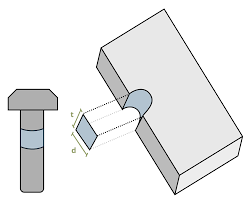
\includegraphics[width=0.80in]{image1.png}};
\end{tikzpicture}

\begin{minipage}{0.95\linewidth}
\sectiontitleOld{Bearing Stress}
$\sigma_B = \dfrac{V}{\text{Projected Area}}$\\[2pt]
$\sigma_{\text{gross}}$: normal stress on full area\\
$\sigma_{\text{net}}$: stress at smallest area
\end{minipage}



\sectiontitleOld{Stress on Oblique Plane}

\begin{tabular}{@{}ll@{}}
$\sigma = \dfrac{P}{A}\cos^{2}\!\theta$ \\
$\tau = \dfrac{P}{A}\sin\theta\cos\theta$
\end{tabular}

\vspace{2pt}
$\sigma_{\text{max}}$: $\theta = 0^\circ$\\
$\tau_{\text{max}}$: $\theta = \pm 45^\circ$


\sectiontitleOld{Factor of Safety}

\[
FS = \frac{\sigma_{\text{ultimate}}}{\sigma_{\text{allowable}}}
\]

\sectiontitleOld{Shear Strain}

$\gamma > 0$: inside angle decreases
\[
\gamma = \theta_{\text{initial}} - \theta_{\text{final}}
\]

\sectiontitleOld{Thermal Deformation}

\[
\delta = \alpha \cdot \Delta T \cdot L
\]

\sectiontitleOld{3D Stress--Strain}

$E\varepsilon_x = \sigma_x - \nu(\sigma_y + \sigma_z)$\\
$E\varepsilon_y = \sigma_y - \nu(\sigma_x + \sigma_z)$\\
$E\varepsilon_z = \sigma_z - \nu(\sigma_x + \sigma_y)$

\vspace{2pt}
\subsectiontitleOld{Poisson Ratio}
\[
\nu = -\frac{\varepsilon_{\text{lateral}}}{\varepsilon_{\text{axial}}}
\]

\subsectiontitleOld{Dilatation (Unit Volume Change)}
\vspace{-10pt}
{\footnotesize\begin{align*}
e &= \varepsilon_x + \varepsilon_y + \varepsilon_z \\
v &= (1+\varepsilon_x)(1+\varepsilon_y)(1+\varepsilon_z) \approx 1 + e \\
e &= v - 1
\end{align*}}
$e$: unit change in volume
\[
e = \frac{1-2\nu}{E}\left(\sigma_x + \sigma_y + \sigma_z\right)
\]

\subsectiontitleOld{Hydrostatic Pressure $p$}
\[
e = -\frac{3(1-2\nu)}{E}\,p
\]

\subsectiontitleOld{Bulk Modulus / Modulus of Compression}
\[
k = \frac{E}{3(1-2\nu)}, \qquad e = -\frac{p}{k}
\]
\[
G = \frac{E}{2(1+\nu)}
\]

\sectiontitleOld{Saint-Venant Principle}

At distance $\geq$ width of member, stress distribution is uniform whether plate-loaded or point-loaded.

\columnbreak

\sectiontitleOld{Stress Concentration}

\[
K = \frac{\sigma_{\max}}{\sigma_{\text{avg}}}
\]

\textbf{Torsion:}
\[
\tau_{\max} = K\left(\frac{Tc}{J}\right)_{\!\text{smaller shaft}}
\]

\sectiontitleOld{Torsion \& Shear Strain}

\begin{tabular}{@{}ll@{}}
$\gamma = \dfrac{\rho\,\phi}{L}$ &
\raisebox{-0.4\height}{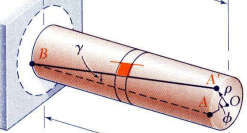
\includegraphics[width=0.65in]{image2.png}}
\end{tabular}

\vspace{3pt}
\begin{tabular}{@{}ll@{}}
$\tau = \dfrac{T\rho}{J}$ &
\raisebox{-0.4\height}{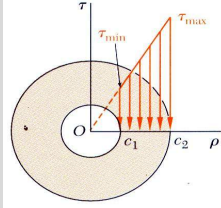
\includegraphics[width=0.5in]{image3.png}}
\end{tabular}

\vspace{2pt}
$\phi = \dfrac{TL}{GJ}$

\vspace{4pt}
\sectiontitleOld{Polar Moment of Inertia}

\[
J_{\text{circle}} = \frac{\pi}{2}r^{4} = \frac{\pi}{32}d^{4}
\]

\vspace{-4pt}


\sectiontitleOld{Gear Ratios}

\[
\frac{T_1}{R_1} = \frac{T_2}{R_2}, \qquad \phi_1 R_1 = \phi_2 R_2
\]

\vspace{-4pt}
\sectiontitleOld{Power}

\[
P = T\omega = 2\pi f T
\]
\begin{align*}
1\;\text{W} &= 1\;\tfrac{\text{N}\cdot\text{m}}{\text{s}} \\
1\;\text{hp} &= 550\;\tfrac{\text{ft}\cdot\text{lb}}{\text{s}}
\end{align*}

\vspace{-4pt}
\sectiontitleOld{Variable Cross-Section}

\[
\phi = \int_{0}^{L}\frac{T}{GJ}\,dx
\]

\[
\phi_{E/B} = \phi_E - \phi_B
\]
(E moves w.r.t.\ B)

\vspace{4pt}
\sectiontitleOld{Modulus of Rupture in Torsion}

\[
R_T = \frac{T_U c}{J}
\]

\vspace{-4pt}
\sectiontitleOld{Plastic Torsion}
\subsectiontitleOld{Not Yield}
\[T = \frac{J}{c}\,\tau_{\max}\]
\subsectiontitleOld{Yield}
\[
T_Y = \frac{J}{c}\,\tau_y = \frac{\pi}{2}\,c^3 \tau_Y
\]

{\footnotesize\begin{tabular}{@{}p{0.4\linewidth}p{0.5\linewidth}@{}}
$0 \le \rho \le \rho_Y$: & $\rho_Y \le \rho \le c$: \\[3pt]
{\scriptsize$\tau = \dfrac{\tau_Y}{\rho_Y}\rho$} &
{\scriptsize$\tau = \tau_Y$} \\[6pt]
\end{tabular}}

{\footnotesize\[
T = \iint \rho\,\tau\,dA = 2\pi\int_{a}^{b}\tau\,\rho^2\,d\rho
\]}

$T_{E-P} = \dfrac{4}{3}T_Y\left(1 - \dfrac{1}{4}\dfrac{\rho_Y^3}{c^3}\right)$\\
$\phi = \frac{\gamma_Y L}{\rho_Y} = \frac{\tau_Y L}{\rho_Y G}$\\
$T_P = \dfrac{4}{3}T_Y$


$\dfrac{\rho_Y}{c} = \dfrac{\phi_Y}{\phi}$ \\
{\footnotesize $\phi_Y$ = angle when outer starts yielding}





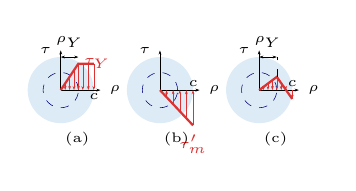
\begin{tikzpicture}[>={Stealth[length=1.5pt, width=1pt]}, scale=0.28, font=\tiny]
\definecolor{shaftblue}{RGB}{220, 235, 245}
\definecolor{stressred}{RGB}{220, 50, 50}
\tikzset{stress arrow/.style={->, stressred, very thin}}
% Figure (a): Loading
\begin{scope}[shift={(0,0)}]
    \fill[shaftblue] (0,0) circle (1.5);
    \draw[dashed, blue!50!black, very thin] (0,0) circle (0.8);
    \draw[->, very thin] (0,0) -- (1.8,0) node[right] {$\rho$};
    \draw[->, very thin] (0,0) -- (0,1.8) node[left] {$\tau$};
    \draw[stressred, thick] (0,0) -- (0.8,1.2) -- (1.5,1.2);
    \foreach \x in {0.2, 0.4, 0.6, 0.8, 1.0, 1.25, 1.5} {
        \draw[stress arrow] (\x, {\x <= 0.8 ? 1.5*\x : 1.2}) -- (\x,0);
    }
    \node[stressred] at (1.65, 1.2) {$\tau_Y$};
    \draw[<->, very thin] (0,1.5) -- (0.8,1.5) node[midway, above] {$\rho_Y$};
    \node at (1.5,-0.3) {$c$};
    \node at (0.75, -2.2) {(a)};
\end{scope}
%\node at (3.5, 0) {\scriptsize \bfseries \textcolor{stressred}{+}};
% Figure (b): Elastic Unloading
\begin{scope}[shift={(4.5,0)}]
    \fill[shaftblue] (0,0) circle (1.5);
    \draw[dashed, blue!50!black, very thin] (0,0) circle (0.8);
    \draw[->, very thin] (0,0) -- (1.8,0) node[right] {$\rho$};
    \draw[->, very thin] (0,0) -- (0,1.8) node[left] {$\tau$};
    \draw[stressred, thick] (0,0) -- (1.5,-1.6);
    \foreach \x in {0.3, 0.6, 0.9, 1.2, 1.5} {
        \draw[stress arrow] (\x, -1.066*\x) -- (\x,0);
    }
    \node[stressred, anchor=north] at (1.5, -1.6) {$\tau'_m$};
    \node at (1.5, 0.3) {$c$};
    \node at (0.75, -2.2) {(b)};
\end{scope}
%\node at (10.5, 0) {\scriptsize \bfseries \textcolor{stressred}{=}};
% Figure (c): Residual Stress
\begin{scope}[shift={(9,0)}]
    \fill[shaftblue] (0,0) circle (1.5);
    \draw[dashed, blue!50!black, very thin] (0,0) circle (0.8);
    \draw[->, very thin] (0,0) -- (1.8,0) node[right] {$\rho$};
    \draw[->, very thin] (0,0) -- (0,1.8) node[left] {$\tau$};
    \draw[stressred, thick] (0,0) -- (0.8, 0.6) -- (1.5, -0.4);
    \foreach \x in {0.2, 0.4, 0.6, 0.8} {
        \draw[stress arrow] (\x, 0.75*\x) -- (\x,0);
    }
    \foreach \x in {1.0, 1.2, 1.5} {
        \pgfmathsetmacro{\yval}{0.6 - (\x-0.8)*1.42}
        \ifdim \yval pt > 0pt
            \draw[stress arrow] (\x, \yval) -- (\x,0);
        \else
            \draw[stress arrow] (\x, 0) -- (\x, \yval);
        \fi
    }
    \draw[dashed, very thin] (0.8, 0.6) -- (0.8, 1.5);
    \draw[<->, very thin] (0,1.5) -- (0.8,1.5) node[midway, above] {$\rho_Y$};
    \node at (1.5, 0.3) {$c$};
    \node at (0.75, -2.2) {(c)};
\end{scope}
\end{tikzpicture}

\vspace{-4pt}
\sectiontitleOld{Torsion Rectangular}
\vspace{-9pt}
\[
\tau_{\max} = \frac{T}{c_1 a b^2} \qquad \phi = \frac{TL}{c_2 a b^3 G}
\]

\columnbreak









\subsectiontitleOld{Residual Shear Strain}
{\footnotesize\[
\phi_r = \phi - \phi' = \frac{\gamma_Y L}{\rho_Y} - \frac{TL}{JG},G = \frac{\tau_Y}{\gamma_Y}
\]}

\sectiontitleOld{Thin-Walled Hollow Shafts}

\[
\tau = \frac{T}{2t\mathcal{A}}, \qquad q = \tau t
\]
\[
\phi = \frac{TL}{4\mathcal{A}^2 G}\oint \frac{ds}{t} \quad \left(\sum_{i=1}^{n} \frac{s_i}{t_i}\right)
\]

$\mathcal{A}$: area enclosed by centerline

\begin{tikzpicture}[remember picture, overlay]
\node[opacity=0.7, anchor=north east] (image) at (\linewidth,-10pt) {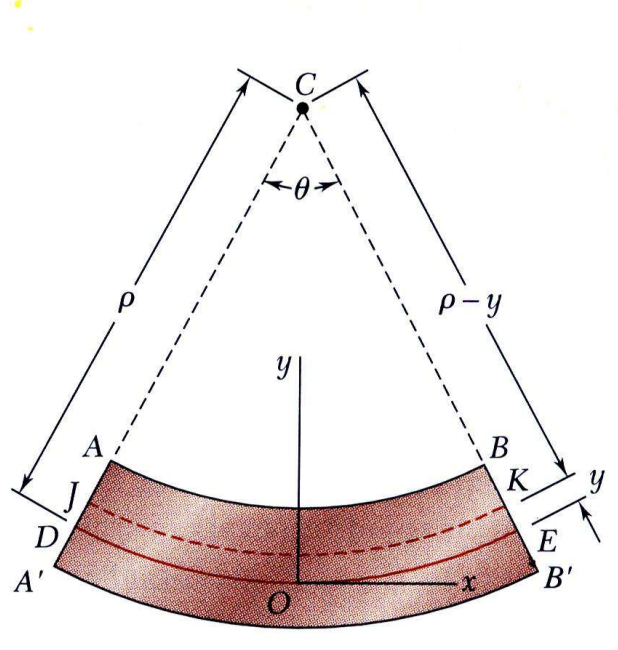
\includegraphics[width=0.8in]{image6.png}};
\end{tikzpicture}

\sectiontitleOld{Pure Bending}

\[
\varepsilon_x = -\frac{y}{\rho}, \varepsilon_{\max} = \frac{c}{\rho}
\]
\[
\sigma_x = -\frac{y}{c}\,E\varepsilon_{\max} = -\frac{y}{c}\,\sigma_{\max}
\]

Neutral axis must pass through the centroid.

\[
\sigma_x = -\frac{My}{I},\sigma_{\max} = \frac{Mc}{I} = \frac{M}{S}
\]

\vspace{4pt}
\sectiontitleOld{Moment of Inertia}

\begin{tabular}{@{}l@{\hspace{2pt}}l@{}}
Rectangle: & $I = \dfrac{1}{12}bh^3$ \\[6pt]
Circle: & $I = \dfrac{\pi}{4}r^4$ \\[6pt]
Parallel axis: & $I = I_{CM} + Ad^2$
\end{tabular}

\vspace{2pt}
$S = \dfrac{I}{c}$ --- section modulus

Rectangle: $S = \dfrac{1}{6}bh^2$



\begin{tikzpicture}[remember picture, overlay]
\node[opacity=0.7, anchor=north east] (image) at (\linewidth,-10pt) {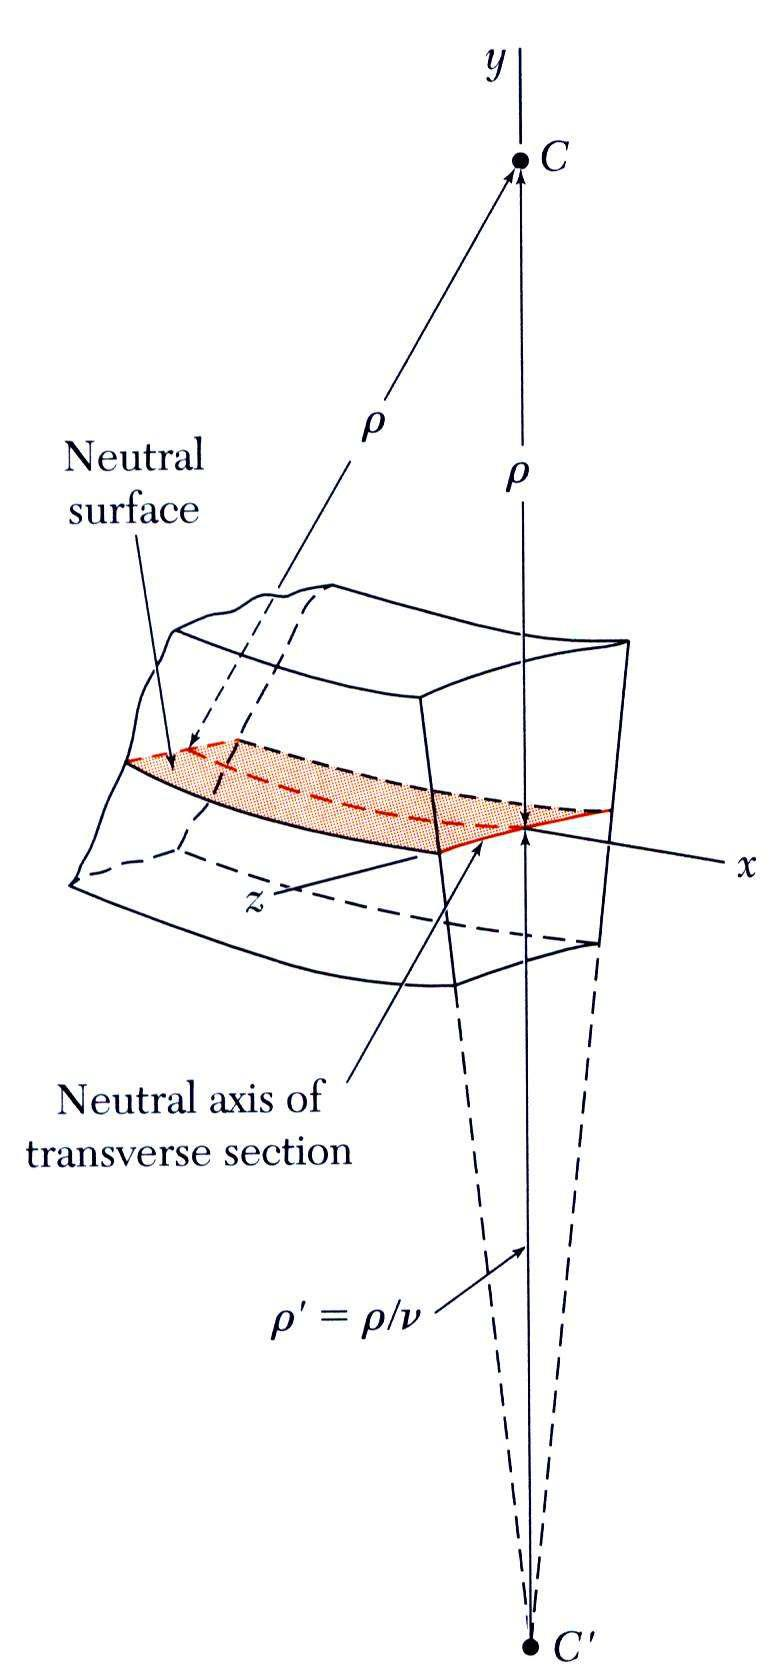
\includegraphics[width=0.6in]{image7.png}};
\end{tikzpicture}

\sectiontitleOld{Curvature}

\[
\frac{1}{\rho} = \frac{\varepsilon_{\max}}{c} = \frac{\sigma_{\max}}{Ec} = \frac{M}{EI}
\]

\subsectiontitleOld{Anticlastic Curvature $\rho'$}
\[
\varepsilon_y = \varepsilon_z = -\nu\varepsilon_x = \frac{\nu y}{\rho},
\frac{1}{\rho'} = \frac{\nu}{\rho}
\]


\sectiontitleOld{Composite Materials}

Replace higher-$E$ material with low-$E$ material but multiply the width by $n = \dfrac{E_2}{E_1}$.\\
Multiply stress by $n$ for stiff material.
\vspace{-4pt}

\begin{center}
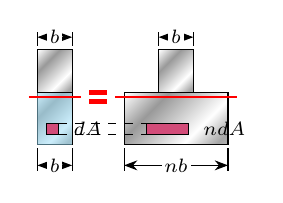
\begin{tikzpicture}[scale=0.22,
    shiny_grey/.style={draw=black, shading=chrome_shine, shading angle=135},
    shiny_blue/.style={draw=black, shading=chrome_shine, shading angle=135, postaction={fill=cyan!40, opacity=0.5}},
    dim_line/.style={{Stealth}-{Stealth}, thin},
    every node/.style={font=\scriptsize}
]
    % LEFT FIGURE
    \draw[shiny_grey] (0,3) rectangle (2,5.5);
    \draw[shiny_blue] (0,0) rectangle (2,3);
    \draw (0,5.7) -- (0,6.5); \draw (2,5.7) -- (2,6.5);
    \draw[dim_line] (0,6.2) -- node[fill=white, inner sep=1pt] {$b$} (2,6.2);
    \draw (0,-0.2) -- (0,-1.5); \draw (2,-0.2) -- (2,-1.5);
    \draw[dim_line] (0,-1.2) -- node[fill=white, inner sep=1pt] {$b$} (2,-1.2);
    \filldraw[fill=purple!70, draw=black] (0.5, 0.6) rectangle (1.2, 1.2);
    \node[right=2pt] at (1.2, 0.9) {$dA$};
    % EQUALS
    \draw[red, line width=1.7pt] (3.0, 3.0) -- (4.0, 3.0);
    \draw[red, line width=1.7pt] (3.0, 2.5) -- (4.0, 2.5);
    % RIGHT FIGURE
    \draw[shiny_grey] (7, 3) rectangle (9, 5.5);
    \draw[shiny_grey] (5, 0) rectangle (11, 3);
    \draw (7,5.7) -- (7,6.5); \draw (9,5.7) -- (9,6.5);
    \draw[dim_line] (7,6.2) -- node[fill=white, inner sep=1pt] {$b$} (9,6.2);
    \draw (5,-0.2) -- (5,-1.5); \draw (11,-0.2) -- (11,-1.5);
    \draw[dim_line] (5,-1.2) -- node[fill=white, inner sep=1pt] {$nb$} (11,-1.2);
    \filldraw[fill=purple!70, draw=black] (6.3, 0.6) rectangle (8.7, 1.2);
    \node[right=2pt] at (8.7, 0.9) {$ndA$};
    % ANNOTATIONS
    \draw[red, thick] (-0.5, 2.75) -- (2.5, 2.75);
    \draw[red, thick] (4.5, 2.75) -- (11.5, 2.75);
    \draw[dashed, thin] (1.2, 1.2) -- (6.3, 1.2);
    \draw[dashed, thin] (1.2, 0.6) -- (6.3, 0.6);
    \draw[dashed] (7,3) -- (9,3);
\end{tikzpicture}
\end{center}
\vspace{-10pt}

\sectiontitleOld{Stress Concentration (Bending)}

\[
\sigma_{\max} = K\!\left(\frac{Mc}{I}\right)_{\!\text{critical}}
\]

\vspace{4pt}
\sectiontitleOld{Modulus of Rupture in Bending}

\[
R_B = \frac{M_U c}{I}
\]

\vspace{4pt}
\sectiontitleOld{Plastic Bending}
\subsectiontitleOld{Not Yield}
\vspace{-10pt}

\[ M = \frac{\sigma_{\max} I}{c} \]

\subsectiontitleOld{Yield}
\vspace{-10pt}
{\footnotesize\[
M_Y = \frac{I}{c}\,\sigma_Y = \frac{2}{3}bc^2 \sigma_Y
\]}

{\footnotesize\begin{tabular}{@{}p{0.4\linewidth}p{0.5\linewidth}@{}}
$0 \le |y| \le y_Y$: &
$y_Y \le |y| \le c$: \\[3pt]
$\sigma = -\dfrac{\sigma_Y}{y_Y}y$ &
$\sigma = \sigma_Y$ 
\end{tabular}}

{\footnotesize\[
M = \iint y\,\sigma\,dA = 2b\int_0^c \sigma\,y\,dy
\]

$M_{E-P} = \frac{3}{2} M_Y \left(1 - \dfrac{y_Y^2}{3c^2}\right)$\\
$\frac{1}{\rho} = \frac{\varepsilon_Y}{y_Y}$\\
$M_P = \dfrac{3}{2}M_Y$
}

\subsectiontitleOld{Residual Curvature}
{\footnotesize\[
\frac{1}{\rho_r} = \frac{1}{\rho} - \frac{1}{\rho'} 
= \frac{\varepsilon_Y}{y_Y} - \frac{M}{EI}
\]}

\vspace{2pt}
\hrule height 0.3pt
\vspace{2pt}

{\footnotesize\begin{tabular}{@{}m{0.45\linewidth}m{0.45\linewidth}@{}}
$Z = \dfrac{M_p}{\sigma_Y}$ & (plastic section modulus) \\[8pt]
$k = \dfrac{M_p}{M_Y} = \dfrac{Z}{S}$ & (shape factor)
\end{tabular}}

\begin{center}
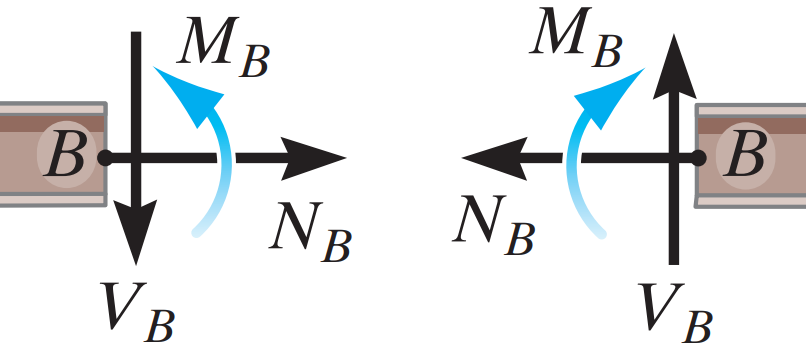
\includegraphics[width=1.5in]{image9.png}
\end{center}

\vspace{4pt}


\begin{tikzpicture}[remember picture, overlay]
\node[opacity=0.7, anchor=north west] (image) at (0,-1.0cm) {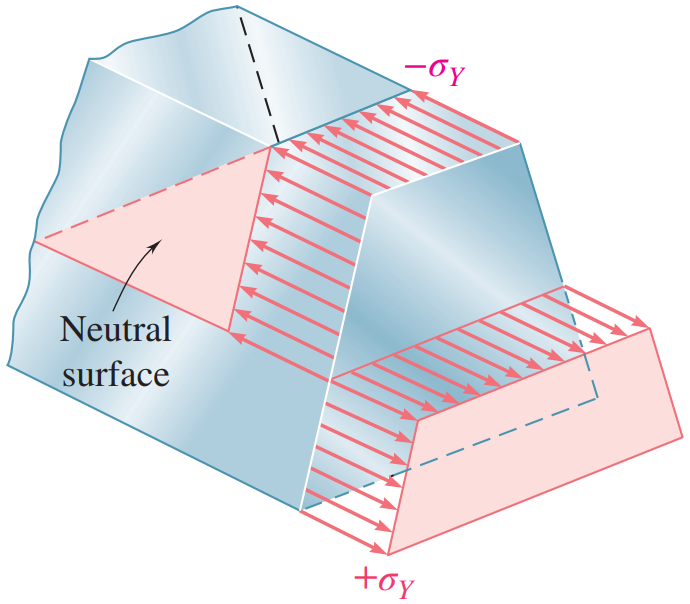
\includegraphics[width=0.50in]{image35.png}};
\node[opacity=0.7, anchor=north east] (image) at (\linewidth,-1.0cm) {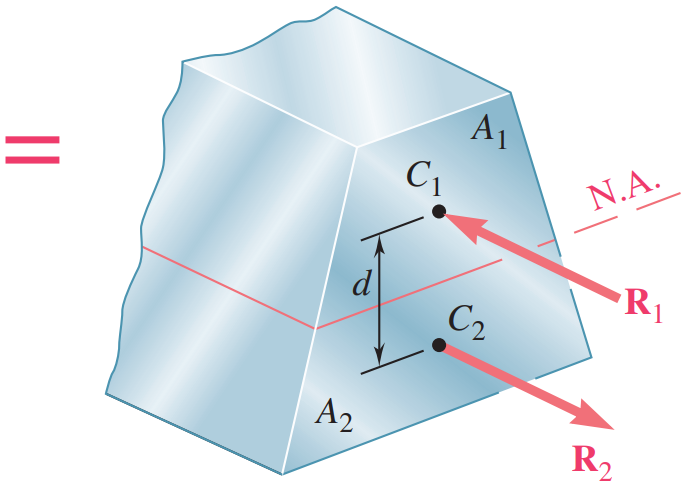
\includegraphics[width=0.50in]{image36.png}};
\end{tikzpicture}

\vspace{-1cm}
\sectiontitleOld{Unsymmetric Cross-Section (Plastic)}

For non-symmetric sections, neutral axis $\neq$ centroidal axis.

\vspace{2pt}
Neutral axis divides cross-section into \textbf{equal areas}.

{\footnotesize
$M_p = \left(\dfrac{1}{2}A\sigma_Y\right)d$
}


\vspace{2pt}
$d$: distance between tension/compression centroids

\vspace{4pt}

\begin{tikzpicture}[remember picture, overlay]
\node[opacity=0.7, anchor=north east] (image) at (\linewidth+0.5cm,-10pt) {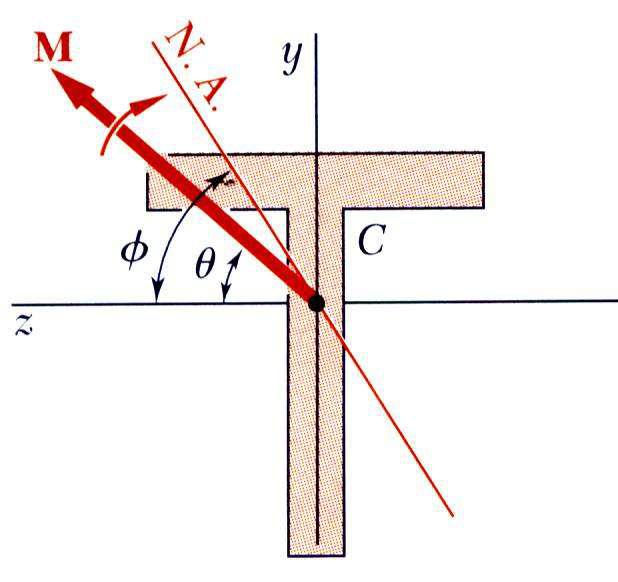
\includegraphics[width=1.0in]{image12.png}};
\node[opacity=0.7, anchor=north east] (image) at (\linewidth,-3cm) {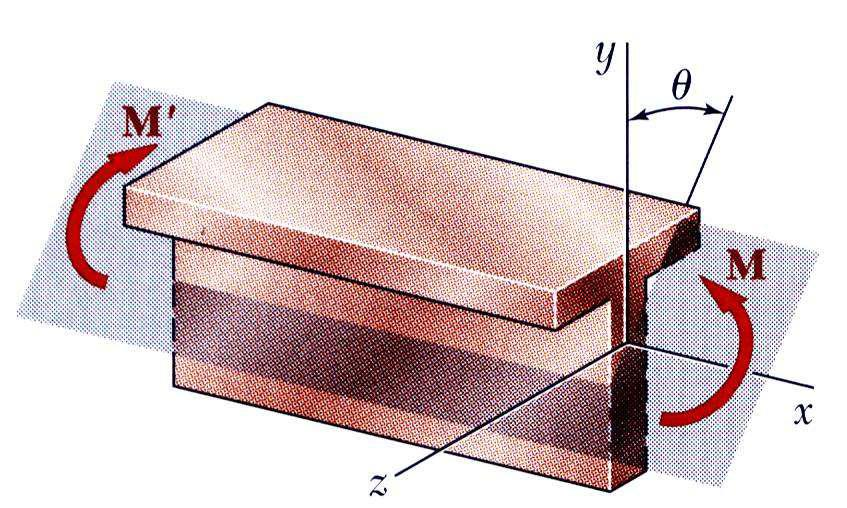
\includegraphics[width=1.0in]{image11.png}};
\node[opacity=0.7, anchor=north east] (image) at (\linewidth,-5cm) {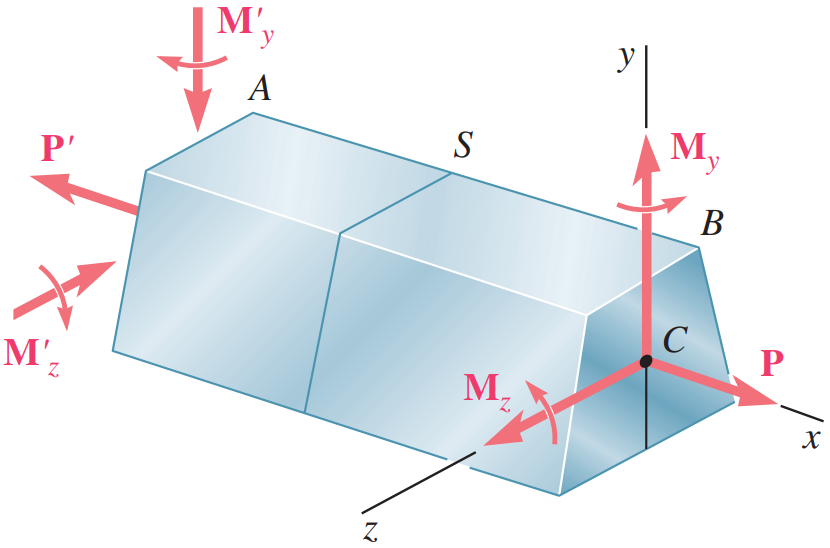
\includegraphics[width=1.0in]{image37.png}};
\end{tikzpicture}

\sectiontitleOld{Unsymmetric Bending}

Resolve moment into principal axes:
\[
M_z = M\cos\theta, M_y = M\sin\theta
\]

Superpose stress distributions:
\[
\sigma = -\frac{M_z y}{I_z} + \frac{M_y z}{I_y}
\]



\begin{minipage}{0.95\linewidth}
\subsectiontitleOld{Neutral axis orientation}

$\tan\phi = \frac{y}{z} = \frac{I_z}{I_y}\tan\theta$

\end{minipage}


\sectiontitleOld{Eccentric Axial Loading}

\[
\sigma_x = \frac{P}{A} - \frac{M_z y}{I_z} + \frac{M_y z}{I_y}
\]

\vspace{2pt}
\textbf{Neutral axis:}
\[
\frac{M_z}{I_z}y - \frac{M_y}{I_y}z = \frac{P}{A}
\]

\columnbreak

\sectiontitle{Elastic Curve}

\[
\frac{1}{\rho} = \frac{d^2y}{dx^2} = \frac{M}{EI}, \quad \frac{d^4y}{dx^4} = \frac{w}{EI}
\]

$M > 0$: sagging\\
$M < 0$: hogging\\
Pin/Roller/Journal/Thrust support: $y = 0$, $y' \neq 0$\\
Fixed support: $y = 0$, $y' = 0$\\
\begin{tabular}{@{}m{0.35\linewidth}@{\hspace{6pt}}m{0.6\linewidth}@{}}
Free End: & $\left\{\begin{array}{l} M = EIy'' = 0 \\[0pt] V = EIy''' = 0 \end{array}\right.$ \\
\end{tabular}
\begin{tabular}{@{}m{0.35\linewidth}@{\hspace{6pt}}m{0.6\linewidth}@{}}
Segments: & $\left\{\begin{array}{l} y_1(a) = y_2(a) \\[0pt] y_1'(a) = y_2'(a) \end{array}\right.$ \\
\end{tabular}
\begin{tabular}{@{}m{0.35\linewidth}@{\hspace{6pt}}m{0.6\linewidth}@{}}
Symmetry: & $\left\{\begin{array}{l} y(\text{center}) = y_{\max} \\[0pt] y'(\text{center}) = 0 \end{array}\right.$ \\
\end{tabular}
Complementary Coordinates:\\
$x_2 = L - x_1$ \\
$y_1'(x_1=a) = - y_2'(x_2=L-a)$

\sectiontitle{Transverse and Longitudinal Shear}
\begin{tabular}{@{}ll@{}} \quad
$\tau = \frac{VQ}{It}$ &
\raisebox{-0.4\height}{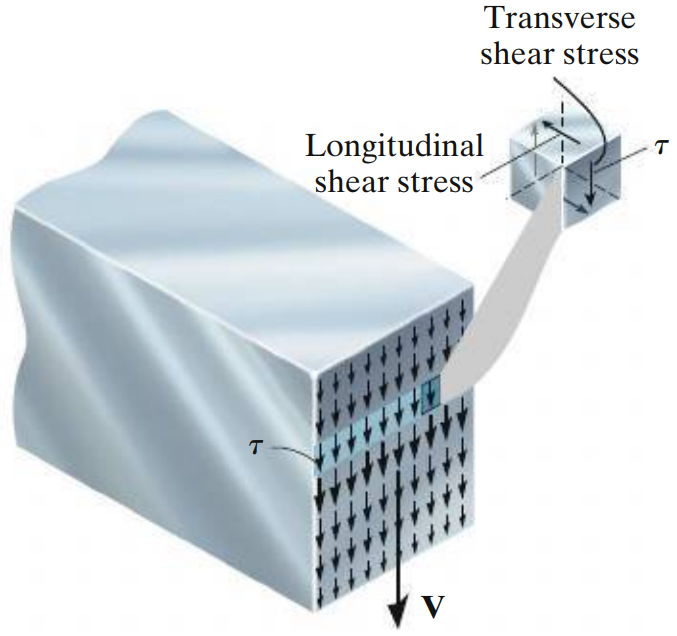
\includegraphics[width=0.65in]{image15.png}}
\end{tabular}


$V$: shear force\\
$Q$: first moment of area\\
$I$: second moment of inertia\\
$t$: width

\subsectiontitle{Narrow Rectangular Beam}
\vspace{-5pt}
\[
\tau_{xy} = \frac{3P}{2A}\left(1 - \frac{y^2}{c^2}\right)
\]
\vspace{-5pt}
\subsectiontitle{Shear Flow}
\vspace{-15pt}

\[
q = \frac{VQ}{I}
\]
\vspace{-5pt}
\subsectiontitle{Force for One Nail}
\vspace{-2pt}
\[
F_{\text{nail}} = \frac{q \cdot s}{n}
\]
\scriptsize{
$\left(\frac{\text{Force}}{\text{Length}} \cdot \frac{\text{Length}}{\text{Nail}} \div \text{rows} = \frac{\text{Force}}{\text{Nail}}\right)$
}
$s$: spacing between nails \\
$n$: number of rows of nails

\subsectiontitle{Unsymmetric Beam / Shear Center}
\[
F = \int_A^B q \, ds, \quad V = \int_B^D q \, ds, \quad e = \frac{Fh}{V}
\]

\begin{center}
\raisebox{-.5\height}{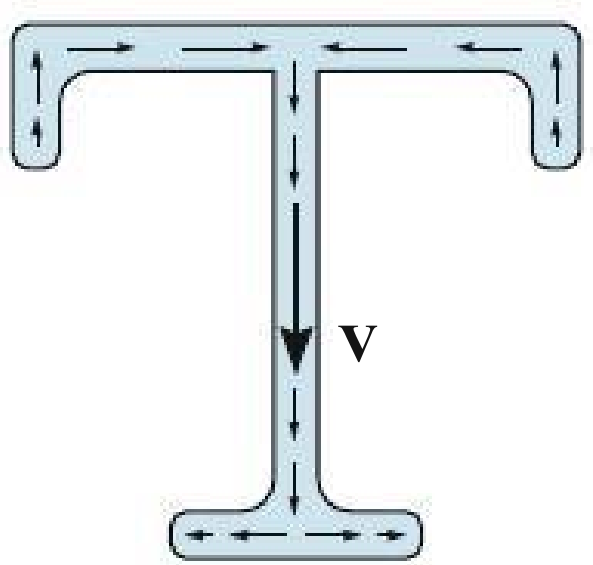
\includegraphics[width=0.6in]{image16.png}} \hspace{10pt} \raisebox{-.5\height}{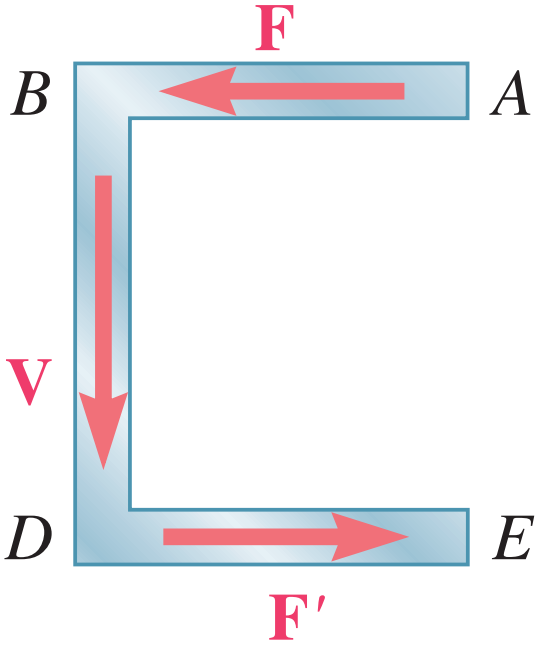
\includegraphics[width=0.6in]{image26.png}}
\end{center}
\vspace{-5pt}

\begin{center}
\raisebox{-.5\height}{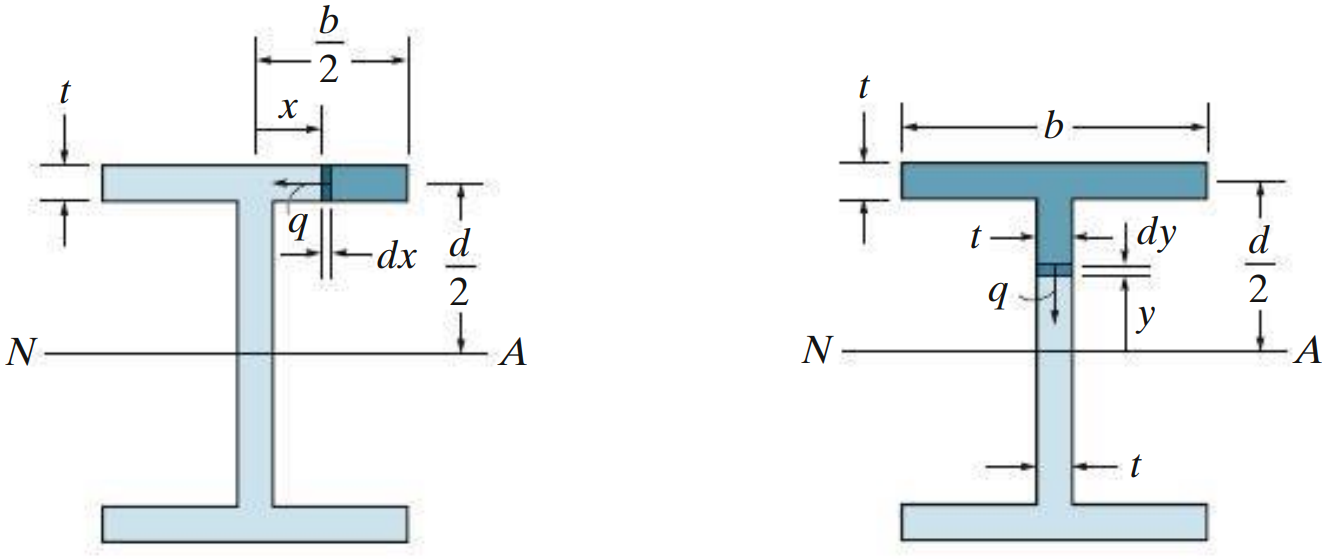
\includegraphics[width=1in]{image17.png}} \hspace{10pt} \raisebox{-.5\height}{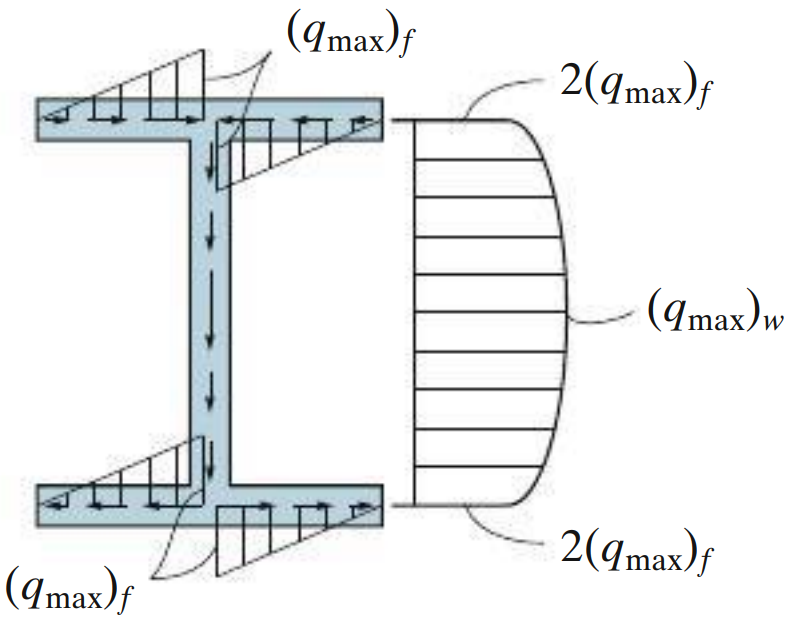
\includegraphics[width=1in]{image18.png}}
\end{center}
\vspace{-5pt}

\subsectiontitle{Composite Section}
\[ 
\tau = \frac{VQ_{\text{tr}}}{I_{\text{tr}}t_{\text{actual}}}
\]

\subsectiontitleOld{Geometry}
\[
\bar{y}_{\text{half-circle}} = \frac{4r}{3\pi}
\]

\end{multicols*}

\newpage

%% ============================================================
%% PAGE 2
%% ============================================================

\begin{multicols*}{3}
\raggedcolumns

%% COLUMN 1





\sectiontitle{Transformations of Plane Stress}
\vspace{-2pt}
Let $\sigma_{\text{avg}} = \dfrac{\sigma_x+\sigma_y}{2}$, $R = \sqrt{\left(\dfrac{\sigma_x-\sigma_y}{2}\right)^{\!2}+\tau_{xy}^2}$
\vspace{-4pt}
{\footnotesize\begin{align*}
\sigma_{x'} &= \sigma_{\text{avg}} + \tfrac{\sigma_x-\sigma_y}{2}\cos 2\theta + \tau_{xy}\sin 2\theta \\
\sigma_{y'} &= \sigma_{\text{avg}} - \tfrac{\sigma_x-\sigma_y}{2}\cos 2\theta - \tau_{xy}\sin 2\theta \\
\tau_{x'y'} &= -\tfrac{\sigma_x-\sigma_y}{2}\sin 2\theta + \tau_{xy}\cos 2\theta \\
\sigma_{x'} + \sigma_{y'} &= \sigma_x + \sigma_y
\end{align*}}
\vspace{-6pt}
$\tan 2\theta_p = \dfrac{2\tau_{xy}}{\sigma_x - \sigma_y}$, \quad $\sigma_{\max,\min} = \sigma_{\text{avg}} \pm R$\\[3pt]
\\[1pt]
$\tan 2\theta_s = -\dfrac{\sigma_x - \sigma_y}{2\tau_{xy}}$, \quad $\tau_{\max} = R$, \quad $\sigma' = \sigma_{\text{avg}}$
\\[3pt]
\text{$\theta_{p1}$ brings the $x$ face to $\sigma_{\max}$ (principal plane)}

\sectiontitle{Transformations of Plane Strain}
\vspace{-2pt}
Let $\varepsilon_{\text{avg}} = \dfrac{\varepsilon_x+\varepsilon_y}{2}$, $R = \sqrt{\left(\dfrac{\varepsilon_x-\varepsilon_y}{2}\right)^{\!2}+\left(\dfrac{\gamma_{xy}}{2}\right)^2}$
\vspace{-4pt}
{\footnotesize\begin{align*}
\varepsilon_{x'} &= \varepsilon_{\text{avg}} + \tfrac{\varepsilon_x-\varepsilon_y}{2}\cos 2\theta + \tfrac{\gamma_{xy}}{2}\sin 2\theta \\
\varepsilon_{y'} &= \varepsilon_{\text{avg}} - \tfrac{\varepsilon_x-\varepsilon_y}{2}\cos 2\theta - \tfrac{\gamma_{xy}}{2}\sin 2\theta \\
\tfrac{\gamma_{x'y'}}{2} &= -\tfrac{\varepsilon_x-\varepsilon_y}{2}\sin 2\theta + \tfrac{\gamma_{xy}}{2}\cos 2\theta \\
\varepsilon_{x'} + \varepsilon_{y'} &= \varepsilon_x + \varepsilon_y
\end{align*}}
\vspace{-6pt}
$\tan 2\theta_p = \dfrac{\gamma_{xy}}{\varepsilon_x - \varepsilon_y}$, \quad $\varepsilon_{\max,\min} = \varepsilon_{\text{avg}} \pm R$\\[3pt]
\\[1pt]
$\tan 2\theta_s = -\dfrac{\varepsilon_x - \varepsilon_y}{\gamma_{xy}}$, \quad $\tfrac{\gamma_{\max}}{2} = R$, \quad $\varepsilon' = \varepsilon_{\text{avg}}$
\\[3pt]
\text{$\theta_{p1}$ brings the $x$ face to $\varepsilon_{\max}$ (principal plane)}






\sectiontitle{Mohr's Circle}
\vspace{-10pt}

\begin{center}
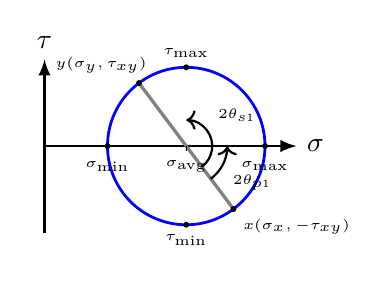
\begin{tikzpicture}[scale=0.2]
\tikzset{prerot/.style={line width=1.2pt,color=gray},
         reflineprerot/.style={line width=0.2pt,color=gray,dashed}}
\def\sigmax{9}\def\sigmay{3}\def\tauxy{4}
\pgfmathsetmacro\sigmam{0.5*(\sigmax+\sigmay)}
\pgfmathsetmacro\sigmad{0.5*(\sigmax-\sigmay)}
\pgfmathsetmacro\r{sqrt((\sigmad)^2+(\tauxy)^2)}
\def\s{0.5}\def\xoff{3}
\pgfmathsetmacro\w{\sigmam+\r+\s}
\pgfmathsetmacro\h{\r+\s}
% Axes
\draw[line width=1pt,-latex](-\xoff,-\h)--(-\xoff,\h) node[at end,anchor=south]{$\tau$};
\draw[line width=1pt,-latex](-\xoff,0)--(\w+1.5,0) node[at end,anchor=west]{$\sigma$};
% Circle
\draw[color=blue,line width=1pt](\sigmam,0) circle (\r);
% Px--Py diameter line
\draw[prerot](\sigmax,-\tauxy)--(\sigmay,\tauxy);
\node at(\sigmax,-\tauxy)[anchor=north west,font=\tiny]{$x(\sigma_x,-\tau_{xy})$};
\node at(\sigmay+4cm,\tauxy)[anchor=south east,font=\tiny]{$y(\sigma_y,\tau_{xy})$};
% add dots at Px and Py
\filldraw[black](\sigmax,-\tauxy) circle(0.15);
\filldraw[black](\sigmay,\tauxy) circle(0.15);


% sigma_m label
\draw(\sigmam,0)--+(0,-0.3) node[anchor=north,font=\tiny]{$\sigma_{\text{avg}}$};
% Principal stress points
\filldraw[black](\sigmam+\r,0) circle(0.15)
  node[anchor=north,font=\tiny,yshift=-2pt]{$\sigma_{\max}$};
\filldraw[black](\sigmam-\r,0) circle(0.15)
  node[anchor=north,font=\tiny,yshift=-2pt]{$\sigma_{\min}$};
% tau_max point (top of circle)
\filldraw[black](\sigmam,\r) circle(0.15)
  node[anchor=south,font=\tiny]{$\tau_{\max}$};
% tau_min point (bottom of circle)
\filldraw[black](\sigmam,-\r) circle(0.15)
  node[anchor=north,font=\tiny]{$\tau_{\min}$};
% Angle computations
\pgfmathsetmacro{\psi}{atan2(-\tauxy,\sigmad)} % angle of Px from center (~-53deg)
% 2*theta_p arc: from Px direction to sigma_max (0 deg)
\draw[->,line width=0.8pt]
  ($(\sigmam,0)+(\psi:0.52*\r)$) arc(\psi:0:0.52*\r)
  node[pos=0.5,anchor=north west,font=\tiny]{$2\theta_{p\scalebox{0.8}{1}}$};
% 2*theta_s arc: from Px direction to tau_max (90 deg)
\draw[->,line width=0.8pt]
  ($(\sigmam,0)+(\psi:0.33*\r)$) arc(\psi:90:0.33*\r)
  node[pos=0.6,anchor=south west,font=\tiny]{$2\theta_{s\scalebox{0.8}{1}}$};
\end{tikzpicture}
\end{center}


\vspace{-10pt}
\sectiontitle{Mohr's Circle --- 3D}
\vspace{-8pt}


\begin{center}
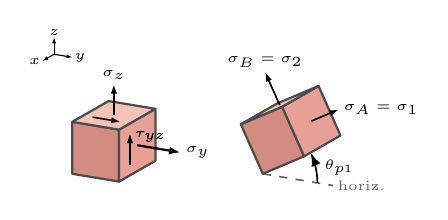
\begin{tikzpicture}[scale=0.22]
    % --- GLOBAL DEFINITIONS ---
    \def\a{3.0} % Cube side length
    \def\shiftx{11} % Shift for second cube

    % Custom colors
    \definecolor{faceleft}{RGB}{210, 140, 130}
    \definecolor{facefront}{RGB}{230, 160, 150}
    \definecolor{facetop}{RGB}{245, 195, 185}

    % Thinner arrows and smaller tips
    \tikzset{
        stressarrow/.style={-{Latex[length=1.2mm, width=0.8mm]}, semithick},
        heavyarrow/.style={-{Latex[length=1.5mm, width=1.0mm]}, thick},
        coordarrow/.style={-{Latex[length=0.8mm, width=0.5mm]}, thin},
        every node/.style={font=\tiny, inner sep=0.5pt}
    }

    % Base projection vectors
    \def\vx{-0.7} \def\vy{-0.4}
    \def\ux{0.9}  \def\uy{-0.15}
    \def\wx{0}    \def\wy{1}

    % CUBE 1
    \begin{scope}[x={(\vx cm,\vy cm)}, y={(\ux cm,\uy cm)}, z={(\wx cm,\wy cm)}]
        \draw[fill=faceleft, draw=black!70, thick, line join=round] (\a,0,0) -- (\a,\a,0) -- (\a,\a,\a) -- (\a,0,\a) -- cycle;
        \draw[fill=facefront, draw=black!70, thick, line join=round] (0,\a,0) -- (\a,\a,0) -- (\a,\a,\a) -- (0,\a,\a) -- cycle;
        \draw[fill=facetop, draw=black!70, thick, line join=round] (0,0,\a) -- (\a,0,\a) -- (\a,\a,\a) -- (0,\a,\a) -- cycle;
        \draw[heavyarrow] (\a/2, \a, \a/2) -- (\a/2, \a+2.8, \a/2) node[right, xshift=1pt] {$\sigma_y$};
        \draw[stressarrow] (\a/2, \a/2, \a) -- (\a/2, \a/2, \a+1.8) node[above, yshift=1pt] {$\sigma_z$};

        \draw[stressarrow] (0.7*\a, 0.2*\a, \a) -- (0.7*\a, 0.8*\a, \a) node[right, pos=0.9, xshift=1pt] {};
        \draw[stressarrow] (0.7*\a, \a, 0.2*\a) -- (0.7*\a, \a, 0.8*\a) node[right, pos=0.9, xshift=1pt] {$\tau_{yz}$};
        % On y face (right), pointing in z direction
        \draw[stressarrow] (0.7*\a, \a, 0.2*\a) -- (0.7*\a, \a, 0.8*\a) node[right, pos=0.9, xshift=1pt] {$\tau_{yz}$};
        \begin{scope}[shift={(1.5*\a, 0, 2.5*\a)}] 
            \draw[coordarrow] (0,0,0) -- (1,0,0) node[left] {$x$};
            \draw[coordarrow] (0,0,0) -- (0,1.2,0) node[right] {$y$};
            \draw[coordarrow] (0,0,0) -- (0,0,1) node[above] {$z$};
        \end{scope}
    \end{scope}

    % CUBE 2
    \pgfmathsetmacro{\thetaP}{28} 
    \pgfmathsetmacro{\ct}{cos(\thetaP)}
    \pgfmathsetmacro{\st}{sin(\thetaP)}
    \pgfmathsetmacro{\uxnew}{\ux*\ct + \wx*\st}
    \pgfmathsetmacro{\uynew}{\uy*\ct + \wy*\st}
    \pgfmathsetmacro{\wxnew}{-\ux*\st + \wx*\ct}
    \pgfmathsetmacro{\wynew}{-\uy*\st + \wy*\ct}

    \begin{scope}[shift={(\shiftx, 0)}]
        \begin{scope}[x={(\vx cm,\vy cm)}, y={(\ux cm,\uy cm)}, z={(\wx cm,\wy cm)}]
            \draw[dashed, semithick, black!60] (\a, 0, 0) -- (\a, 4.5, 0) node[right, xshift=1pt] {horiz.};
            \draw[-latex, semithick, domain=0:\thetaP, samples=20] plot (\a, {3.5*cos(\x)}, {3.5*sin(\x)});
            \node[right, xshift=2pt] at (\a, {3.6*cos(\thetaP/2)}, {3.6*sin(\thetaP/2)}) {$\theta_{p\scalebox{0.8}{1}}$};
        \end{scope}
        \begin{scope}[x={(\vx cm,\vy cm)}, y={(\uxnew cm,\uynew cm)}, z={(\wxnew cm,\wynew cm)}]
            \draw[fill=faceleft, draw=black!70, thick, line join=round] (\a,0,0) -- (\a,\a,0) -- (\a,\a,\a) -- (\a,0,\a) -- cycle;
            \draw[fill=facefront, draw=black!70, thick, line join=round] (0,\a,0) -- (\a,\a,0) -- (\a,\a,\a) -- (0,\a,\a) -- cycle;
            \draw[fill=facetop, draw=black!70, thick, line join=round] (0,0,\a) -- (\a,0,\a) -- (\a,\a,\a) -- (0,\a,\a) -- cycle;
            \draw[stressarrow] (\a/2, \a, \a/2) -- (\a/2, \a+2.0, \a/2) node[right, xshift=1pt] {$\sigma_A=\sigma_1$};
            \draw[stressarrow] (\a/2, \a/2, \a) -- (\a/2, \a/2, \a+2.0) node[above, yshift=1pt] {$\sigma_B=\sigma_2$};
        \end{scope}
    \end{scope}
\end{tikzpicture}
\end{center}

\vspace{-10pt}

\noindent
\begin{minipage}[t]{0.55\linewidth}
\centering
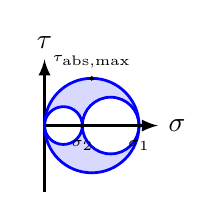
\begin{tikzpicture}[scale=0.12]
\def\siga{10}\def\sigb{4}
\pgfmathsetmacro\rA{0.5*\siga}
\pgfmathsetmacro\rB{0.5*\sigb}
\pgfmathsetmacro\rAB{0.5*(\siga-\sigb)}
\pgfmathsetmacro\cA{\rA}
\pgfmathsetmacro\cB{\rB}
\pgfmathsetmacro\cAB{0.5*(\siga+\sigb)}
\def\s{0.5}\def\xoff{0}
\pgfmathsetmacro\h{\rA+\s+1.5}
% Axes
\draw[line width=1pt,-latex](-\xoff,-\h)--(-\xoff,\h)
  node[at end,anchor=south]{$\tau$};
\draw[line width=1pt,-latex](-\xoff,0)--(\siga+2,0)
  node[at end,anchor=west]{$\sigma$};
% Shading
\fill[blue!15, even odd rule]
  (\cA,0) circle(\rA)
  (\cB,0) circle(\rB)
  (\cAB,0) circle(\rAB);
% Three circles (drawn after so outlines sit on top of shading)
\draw[color=blue,line width=1pt](\cAB,0) circle(\rAB);
\draw[color=blue,line width=1pt](\cB,0) circle(\rB);
\draw[color=blue,line width=1pt](\cA,0) circle(\rA);
% Principal stress points
\filldraw[black](\sigb,0) circle(0.18)
  node[anchor=north,font=\tiny,yshift=-2pt]{$\sigma_2$};
\filldraw[black](\siga,0) circle(0.18)
  node[anchor=north,font=\tiny,yshift=-2pt]{$\sigma_1$};
% tau_abs_max dot and label above circle
\filldraw[black](\cA,\rA) circle(0.18)
  node[anchor=south,font=\tiny]{$\tau_{\text{abs,max}}$};
\end{tikzpicture}
\end{minipage}%
\hfill
\begin{minipage}[t]{0.43\linewidth}
\centering
% Mohr's circles: sigma_1 > 0, sigma_2 < 0 (compression)
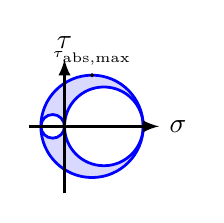
\begin{tikzpicture}[scale=0.1]
\def\siga{10}\def\sigb{-3}
\pgfmathsetmacro\rA{0.5*\siga}
\pgfmathsetmacro\rB{0.5*abs(\sigb)}
\pgfmathsetmacro\rAB{0.5*(\siga-\sigb)}
\pgfmathsetmacro\cA{\rA}
\pgfmathsetmacro\cB{0.5*\sigb}
\pgfmathsetmacro\cAB{0.5*(\siga+\sigb)}
\def\s{0.5}
\pgfmathsetmacro\xoff{abs(\sigb)+1.5}
\pgfmathsetmacro\h{\rAB+\s+1.5}
% Shading (between outer and inner circles)
\fill[blue!15, even odd rule]
  (\cA,0) circle(\rA)
  (\cB,0) circle(\rB)
  (\cAB,0) circle(\rAB);
% Three circles
\draw[color=blue,line width=1pt](\cAB,0) circle(\rAB);
\draw[color=blue,line width=1pt](\cB,0) circle(\rB);
\draw[color=blue,line width=1pt](\cA,0) circle(\rA);
% Axes drawn last so they appear on top
\draw[line width=1pt,-latex](0,-\h)--(0,\h)
  node[at end,anchor=south]{$\tau$};
\draw[line width=1pt,-latex]({-\xoff},0)--(\siga+2,0)
  node[at end,anchor=west]{$\sigma$};

% tau_abs_max dot and label (now at top of largest circle)
\filldraw[black](\cAB,\rAB) circle(0.18)
  node[anchor=south,font=\tiny]{$\tau_{\text{abs,max}}$};
% Mark sigma=0 axis crossing note
% (0 already labeled as \sigma_2)
\end{tikzpicture}
\end{minipage}

\subsectiontitle{2D \& 3D Shear Sign}
{\scriptsize
$(+)$: Face \& arrow both positive or both negative direction\\
$(-)$: Otherwise\\
}
\subsectiontitle{Axis Substitution}
\vspace{-0.5cm}
{\footnotesize
\begin{center}
\begin{tabular}{@{}l@{\hspace{4pt}}l@{}}
\hline
\textbf{Stress Plane} & \textbf{Plot} \\ \hline
$(x,y)$ & \makecell[l]{$(\sigma_x, -\tau_{xy})$ \\ $(\sigma_y, \tau_{xy})$} \\ \hline
$(y,z)$ & \makecell[l]{$(\sigma_y, -\tau_{yz})$ \\ $(\sigma_z, \tau_{yz})$} \\ \hline
$(z,x)$ & \makecell[l]{$(\sigma_z, -\tau_{xz})$ \\ $(\sigma_x, \tau_{xz})$} \\ \hline
\end{tabular}
\end{center}
}


\sectiontitle{Strain Transformations}
\vspace{-10pt}  

\begin{center}
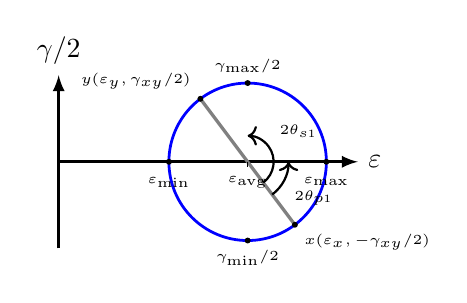
\begin{tikzpicture}[scale=0.2]
\tikzset{prerot/.style={line width=1.2pt,color=gray},
         reflineprerot/.style={line width=0.2pt,color=gray,dashed}}
\def\epsxval{9}\def\epsyval{3}\def\gammaxyval{4}
\pgfmathsetmacro\epsavg{0.5*(\epsxval+\epsyval)}
\pgfmathsetmacro\epsdiff{0.5*(\epsxval-\epsyval)}
\pgfmathsetmacro\r{sqrt((\epsdiff)^2+(\gammaxyval)^2)}
\def\s{0.5}\def\xoff{6}
\pgfmathsetmacro\w{\epsavg+\r+\s}
\pgfmathsetmacro\h{\r+\s}
% Axes
\draw[line width=1pt,-latex](-\xoff,-\h)--(-\xoff,\h) node[at end,anchor=south]{$\gamma/2$};
\draw[line width=1pt,-latex](-\xoff,0)--(\w+1.5,0) node[at end,anchor=west]{$\varepsilon$};
% Circle
\draw[color=blue,line width=1pt](\epsavg,0) circle (\r);
% Px--Py diameter line
\draw[prerot](\epsxval,-\gammaxyval)--(\epsyval,\gammaxyval);
\node at(\epsxval,-\gammaxyval)[anchor=north west,font=\tiny]{$x(\varepsilon_x,-\gamma_{xy}/2)$};
\node at(\epsyval,\gammaxyval)[anchor=south east,font=\tiny]{$y(\varepsilon_y,\gamma_{xy}/2)$};
% add dots at Px and Py
\filldraw[black](\epsxval,-\gammaxyval) circle(0.15);
\filldraw[black](\epsyval,\gammaxyval) circle(0.15);


% eps_avg label
\draw(\epsavg,0)--+(0,-0.3) node[anchor=north,font=\tiny]{$\varepsilon_{\text{avg}}$};
% Principal strain points
\filldraw[black](\epsavg+\r,0) circle(0.15)
  node[anchor=north,font=\tiny,yshift=-2pt]{$\varepsilon_{\max}$};
\filldraw[black](\epsavg-\r,0) circle(0.15)
  node[anchor=north,font=\tiny,yshift=-2pt]{$\varepsilon_{\min}$};
% gamma_max/2 point (top of circle)
\filldraw[black](\epsavg,\r) circle(0.15)
  node[anchor=south,font=\tiny]{$\gamma_{\max}/2$};
% gamma_min/2 point (bottom of circle)
\filldraw[black](\epsavg,-\r) circle(0.15)
  node[anchor=north,font=\tiny]{$\gamma_{\min}/2$};
% Angle computations
\pgfmathsetmacro{\psi}{atan2(-\gammaxyval,\epsdiff)} % angle of Px from center (~-53deg)
% 2*theta_p arc: from Px direction to eps_max (0 deg)
\draw[->,line width=0.8pt]
  ($(\epsavg,0)+(\psi:0.52*\r)$) arc(\psi:0:0.52*\r)
  node[pos=0.5,anchor=north west,font=\tiny]{$2\theta_{p\scalebox{0.8}{1}}$};
% 2*theta_s arc: from Px direction to gamma_max/2 (90 deg)
\draw[->,line width=0.8pt]
  ($(\epsavg,0)+(\psi:0.33*\r)$) arc(\psi:90:0.33*\r)
  node[pos=0.6,anchor=south west,font=\tiny]{$2\theta_{s\scalebox{0.8}{1}}$};
\end{tikzpicture}
\end{center}

\columnbreak

\begin{tikzpicture}[remember picture, overlay]
\node[opacity=1, anchor=north east] (image) at (\linewidth,1.0cm) {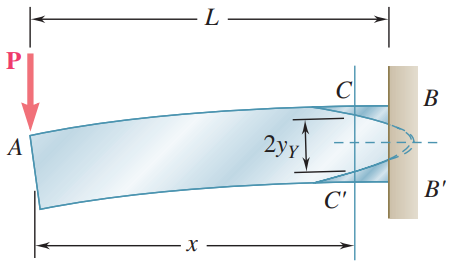
\includegraphics[width=0.80in]{image29.png}};
\node[opacity=1, anchor=north east] (image) at (\linewidth,-1.0cm) {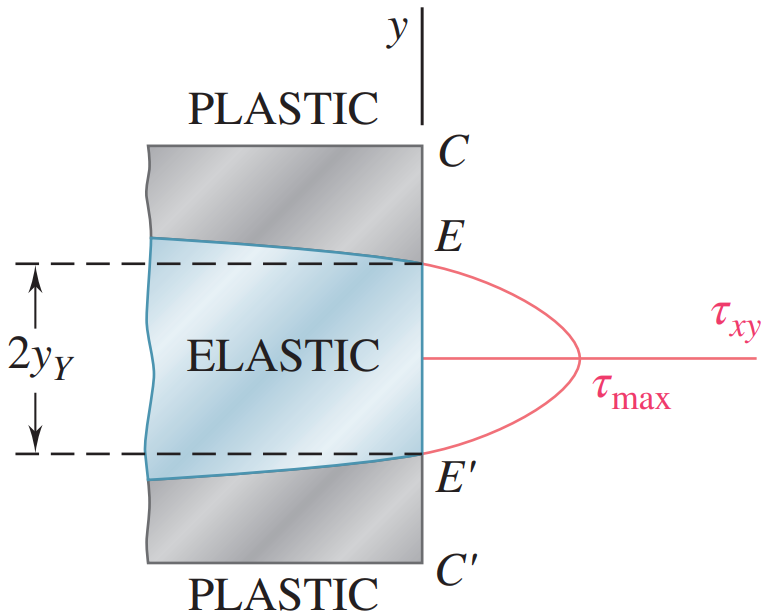
\includegraphics[width=0.80in]{image30.png}};
\end{tikzpicture}


\sectiontitle{Plastic Deformation due to Shear}
$Px = \frac{3}{2}M_Y\left(1 - \frac{y^2}{3 c^2}\right)$\\
$x$: distance from free end\\
\vspace{5pt}
\subsectiontitle{Shear Stress}
$\tau_{xy} = \frac{3}{2}\frac{V}{A'}\left(1 - \frac{y^2}{y_Y^2}\right)$\\
$A'$: area of elastic section\\
$A' = 2by_Y$ for rectangular cross section\\



\begin{tikzpicture}[remember picture, overlay]
\node[opacity=0.7, anchor=north west] (image) at (0,0.5cm) {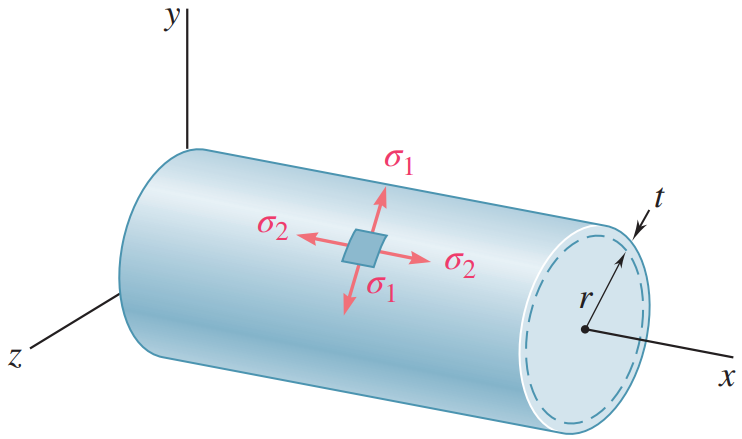
\includegraphics[width=0.80in]{image27.png}};
\node[opacity=0.7, anchor=north east] (image) at (7.0cm,0.5cm) {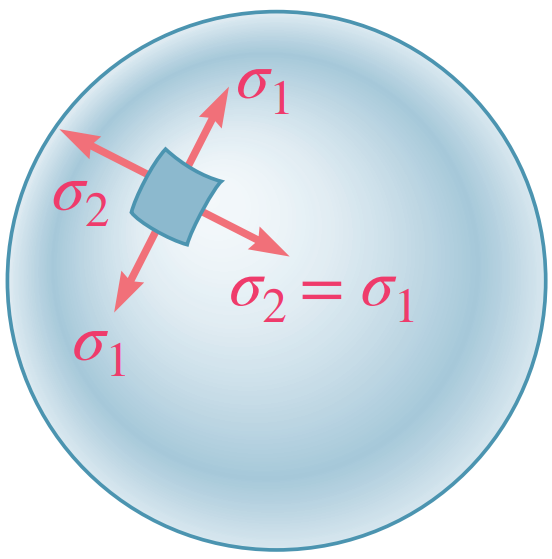
\includegraphics[width=0.50in]{image28.png}};
\end{tikzpicture}
\begin{minipage}{0.95\linewidth}
\sectiontitle{Thin-walled Pressure Vessels}
\[
\sigma_1 = \frac{pr}{t} \text{ (hoop)}, \quad \sigma_2 = \frac{pr}{2t} \text{ (longitudinal)}
\]
\end{minipage}



\sectiontitle{Strain Rosette}
\begin{tikzpicture}[remember picture, overlay]
\node[opacity=0.7, anchor=north] (image) at (0.5\linewidth,0) {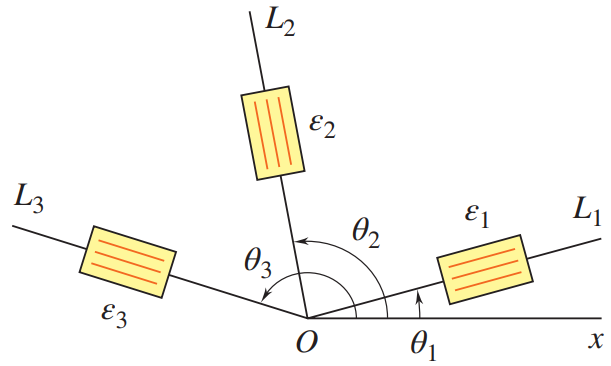
\includegraphics[width=0.60\linewidth]{image25.png}};
\end{tikzpicture}

\[
\varepsilon_1 = \varepsilon_x \cos^2\theta_1 + \varepsilon_y \sin^2\theta_1 + \frac{\gamma_{xy}}{2}\sin 2\theta_1
\]
\[
\varepsilon_2 = \varepsilon_x \cos^2\theta_2 + \varepsilon_y \sin^2\theta_2 + \frac{\gamma_{xy}}{2}\sin 2\theta_2
\]
\[
\varepsilon_3 = \varepsilon_x \cos^2\theta_3 + \varepsilon_y \sin^2\theta_3 + \frac{\gamma_{xy}}{2}\sin 2\theta_3
\]


\vspace{-0.5cm}
\begin{center}
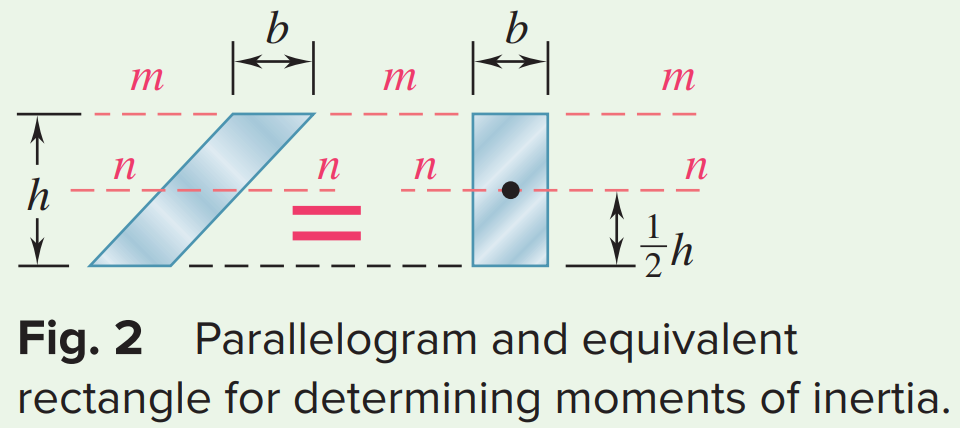
\includegraphics[width=2.0in]{image31.png}
\end{center}
same principle for centroid


\begin{tikzpicture}[remember picture, overlay]
\node[opacity=1.0, anchor=north east] (image) at (\linewidth,0cm) {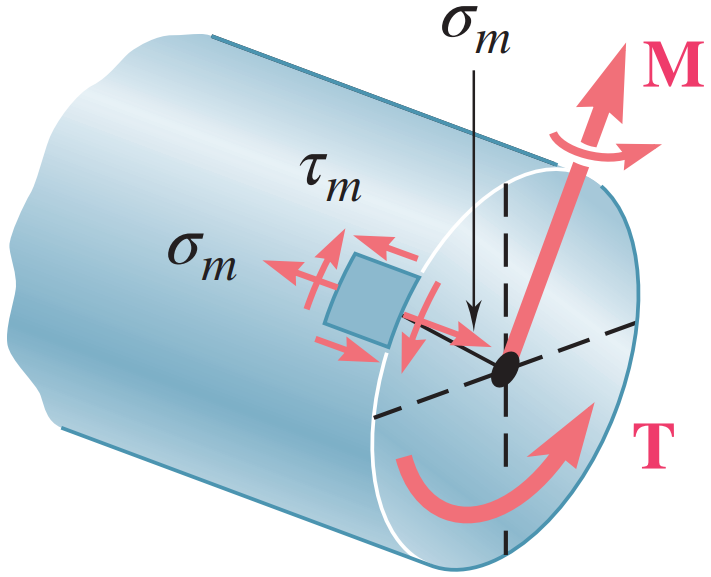
\includegraphics[width=0.60in]{image38.png}};
\end{tikzpicture}

\subsectiontitle{Transmission Shaft Design}

$\tau_{\max} = \frac{c}{J} \sqrt{M_y^2 + M_z^2 + T^2}$


\sectiontitle{Buckling of Columns}
\noindent
\begin{minipage}[c]{0.60\linewidth}
  %{\small
  $P_{cr} = \frac{\pi^2 EI}{L_e^2}, \sigma_{cr} = \frac{\pi^2 E}{(L_e/r)^2}$\\[4pt]
  %}
  {\footnotesize
  $r = \sqrt{I/A}$: radius of gyration\\
  $y_{\max}$ undeterminate for axial load
  }
\end{minipage}%
\hfill
\begin{minipage}[c]{0.35\linewidth}
  \raggedleft\scriptsize
  \raisebox{1pt}[0pt][0pt]{\begin{tabular}{@{}ll@{}}
  \hline
  \textbf{$L_e/L$} & \textbf{Supports} \\ \hline
  1.0 & Pin-Pin \\
  0.5 & Fixed-Fixed \\
  0.7 & Fixed-Pin \\
  2.0 & Fixed-Free \\ \hline
  \end{tabular}}
\end{minipage}


\subsectiontitle{Eccentric Loading}
{\footnotesize
\[ y_{\max} = e \left( \sec{\left( \sqrt{\frac{P}{EI}} \frac{L}{2} \right)} - 1 \right) 
= e \left( \sec{\left( \frac{\pi}{2} \sqrt{\frac{P}{P_{cr}}} \right)} - 1 \right)
\]
}
{\footnotesize
\[
\begin{aligned}
  \sigma_{\max} &= \frac{P}{A} \left( 1 + \frac{(y_{\max}+e)c}{r^2} \right)\\
                &= \frac{P}{A} \left( 1 + \frac{ec}{r^2} \sec{\left( \frac{\pi}{2} \sqrt{\frac{P}{P_{cr}}} \right)} \right)\\
                &= \frac{P}{A} \left( 1 + \frac{ec}{r^2} \sec{\left( \sqrt{\frac{P}{EI}} \frac{L}{2} \right)} \right)
\end{aligned}
\]
}


\sectiontitle{Allowable Stress Design Steel}
\textbf{AB} ($L/r < 4.71\sqrt{E/\sigma_y}$):
$\sigma_{cr} = \left[0.658^{(\sigma_y/\sigma_e)}\right]\sigma_y$,\quad
$\sigma_e = \dfrac{\pi^2 E}{(L/r)^2}$\\
\textbf{BC} ($L/r \geq 4.71\sqrt{E/\sigma_y}$):
$\sigma_{cr} = 0.877\,\sigma_e$\\
\textbf{Allowable:} $\sigma_{all} = \dfrac{\sigma_{cr}}{1.67}$

\textbf{Aluminum Alloys ($\sigma_{all}$)}\\
\textbf{6061-T6:} $L/r<66$: $[20.3-0.127(L/r)]$ ksi $=[140-0.874(L/r)]$ MPa\\
\phantom{\textbf{6061-T6:}} $L/r\geq66$: $\dfrac{51{,}400}{(L/r)^2}$ ksi $=\dfrac{354\times10^3}{(L/r)^2}$ MPa\\
\textbf{2014-T6:} $L/r<55$: $[30.9-0.229(L/r)]$ ksi $=[213-1.577(L/r)]$ MPa\\
\phantom{\textbf{2014-T6:}} $L/r\geq55$: $\dfrac{55{,}400}{(L/r)^2}$ ksi $=\dfrac{382\times10^3}{(L/r)^2}$ MPa

\noindent
\begin{minipage}[t]{0.333\linewidth}\centering\textbf{Steel}\\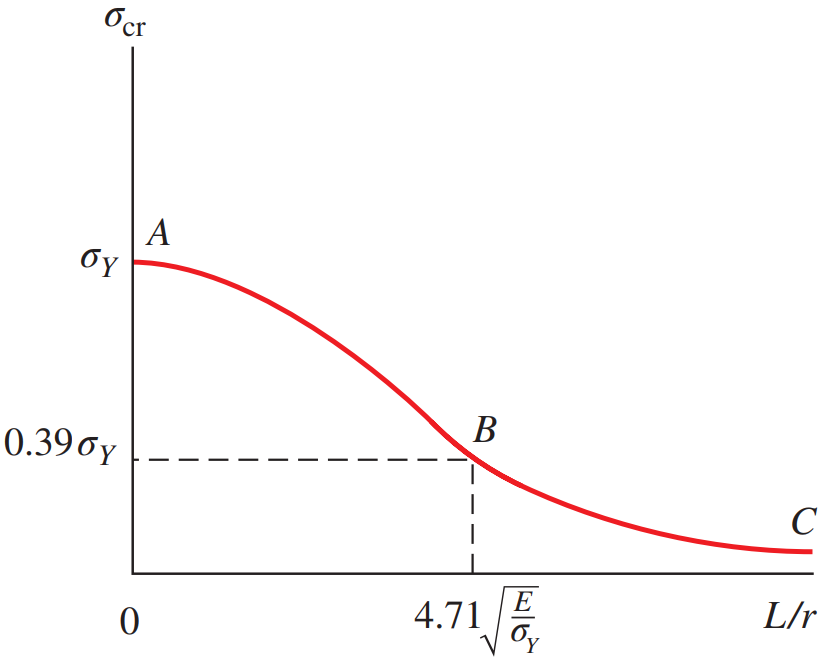
\includegraphics[width=\linewidth]{image39.png}\end{minipage}\hfill
\begin{minipage}[t]{0.333\linewidth}\centering\textbf{Alum.}\\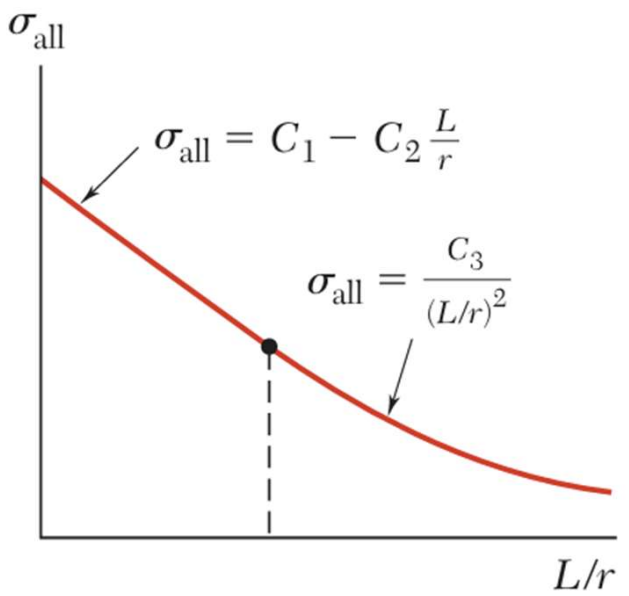
\includegraphics[width=\linewidth]{image40.png}\end{minipage}\hfill
\begin{minipage}[t]{0.333\linewidth}\centering\textbf{Wood}\\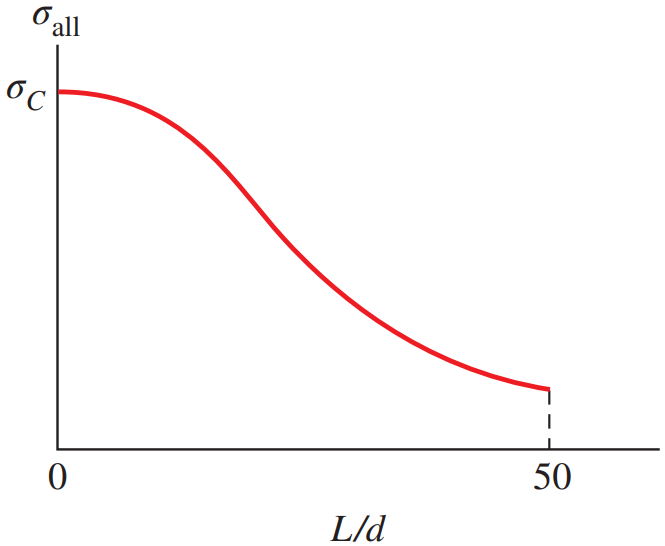
\includegraphics[width=\linewidth]{image41.png}\end{minipage}

\columnbreak

\textbf{Wood (ASD):}
$\sigma_{all}=\sigma_C C_p$,\\
{\small
$C_p=\dfrac{1+(\sigma_{CE}/\sigma_C)}{2c}-\sqrt{\left[\dfrac{1+(\sigma_{CE}/\sigma_C)}{2c}\right]^2-\dfrac{\sigma_{CE}/\sigma_C}{c}}$
}
$\sigma_{CE}=\dfrac{0.822E}{(L/d)^2}$\\
$c=0.8$ (sawn),\ $c=0.9$ (glued laminated wood)\\
$L/d\leq50$

\subsectiontitle{Centric Load Design}
\[ \gamma_D P_D + \gamma_L P_L \leq \phi P_U \]
$P_U = \sigma_{\text{cr}} A$, $\phi = 0.9$ (Steel)

\subsectiontitle{Eccentric Load Design}
\[ \sigma = \sigma_{\text{centric}} + \sigma_{\text{bending}} = \frac{P}{A} + \frac{M c}{I} \leq \sigma_{\text{all}} \]
\subsectiontitle{Interaction Method}
\[ \frac{P/A}{(\sigma_{\text{all}})_{\text{centric}}} + \frac{|M_x| z_{\text{max}} / I_x}{(\sigma_{\text{all}})_{\text{bending}}} + \frac{|M_z| x_{\text{max}} / I_z}{(\sigma_{\text{all}})_{\text{bending}}} \le 1 \]


\end{multicols*}

\end{document}
